\documentclass{article}
\usepackage[utf8]{inputenc}
\usepackage[a4paper,total={6in, 9in}]{geometry}
\usepackage{multicol}
\usepackage{listings}
\usepackage{minted}
\usepackage{graphicx}

\title{Lockatme\\Advancement S3} \author{Pierre-Louis Sergent} \date{\today}

\begin{document}
\begin{titlepage}
  \vspace*{\fill} \begin{center}
  \Huge{Lockatme\\Advancement S3}\\[2.5cm]
  \normalsize{ArchItech Team}\\[3cm]
  \date{\today}
\end{center}
\vspace*{\fill}
\end{titlepage}

  \newpage

  \tableofcontents

  \newpage

  \section{Introduction}

  Lors du S2, le projet Lockatme avait déjà bien avancé, nous avions implémenté
  jusqu’alors un algorithme qui permettait de reconnaître un visage, avec la
  webcam, par rapport à une image passé en paramètre. Ainsi le prototype du S2
  ressemblait à la version final que nous voulions, à l’exception près que nous
  nous contentions d’afficher une image à l’écran, cette dernière disparaissant
  lorsque le visage passé en paramètre était reconnu par la webcam. Le
  développement du projet pour le S3 était donc principalement porté sur
  l’implémentation système, sur le verrouillage et sur l’implémentation d’un
  double déverrouillage, reconnaissance faciale / mot de passe.

  \section{Quelles recherches?}

  L’idée de la reconnaissance faciale nous était venu d’un article de magazine,
  ainsi la documentation sur cette algorithme est très abondante avec de
  multiples solutions. Cependant la partie implémentation système et
  verrouillage sur X11 nous était complètement inconnue il nous fallait donc
  nous plonger dans la recherche et la documentation pour ces deux aspects.
\\ \\
  La première question a été, comment le système gère-t’il le déverrouillage?
\\ \\
  L’ensemble du groupe s’est donc plongé dans cette recherche.

  \section{PAM: Pluggable Authentication Modules} \emph{(Bruno, David,
  Pierre-Louis, travail en parallèle de Python into C)}\\ \\
En nous penchant sur des applications de lock sous Linux, tel que i3lock,
lightDM, nous nous sommes rendu compte qu’elles utilisent toute le module
PAM.
Le module PAM permet à travers de configs files contenant des modules de
gérer l’authentification. Les applications font appels à PAM en passant en
paramètre le nom de la config file, qui elle même contient des modules
d’authentification.

  \begin{figure}[h]
    \begin{center}
    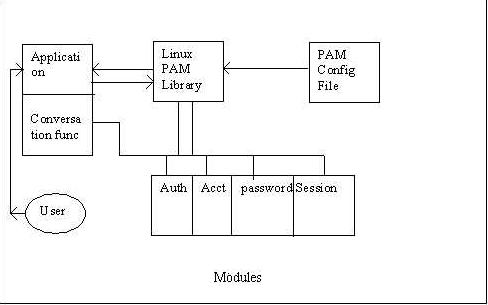
\includegraphics[width=0.8\linewidth]{./pam}
    \caption{schéma explication PAM}
  \end{center}
  \end{figure}

  Nous nous sommes donc réparti les recherches à partir de la en trois parties
  (issues de la documentation officielle):
  \begin{itemize}
    \item{The System Administrators' Guide (Pierre-Louis)}

    \vspace{0.05cm}

Cette partie concerne les PAM config file contenues dans le répertoire
\verb|/etc/pam.d|. Elles contiennent les modules PAM qui seront utilisés suite à
l’appel de PAM par l’application. Il s’agit d’une syntaxe particulière où les
modules sont regroupés en "type groupe" : account, auth, password et session.
Après les types groups, sur la même ligne, vient la "control value", qui va
définir le comportement de l’application en fonction des valeurs de retour des
modules. Par exemple: required, sufficient, include, optional… Après la control
value vient le nom du module PAM utilisé. Ensuite le quatrième argument
constitue des options diverses que nous ne détailleront pas ici car inutile
pour notre projet.
\\ \\
    Exemple: system-auth \\

    auth      required  \texttt{pam\_unix.so}   \texttt{try\_first\_pass
    nullok} \\
    auth      optional  \texttt{pam\_permit.so} \\
    auth      required  \texttt{pam\_env.so} \\

    account   required  \texttt{pam\_unix.so} \\
    account   optional  \texttt{pam\_permit.so} \\
    account   required  \texttt{pam\_time.so} \\

    password  required  \texttt{pam\_unix.so}   \texttt{try\_first\_pass nullok
    sha512 shadow} \\
    password  optional  \texttt{pam\_permit.so} \\

    session   required  \texttt{pam\_limits.so} \\
    session   required  \texttt{pam\_unix.so} \\
    session   optional  \texttt{pam\_permit.so} \\

    \item{The Module Writers' Guide (Bruno)}

    \vspace{0.05cm}

Sur l’exemple du dessus on voit que le troisième argument de chaque ligne est
un module PAM. Il est possible d’écrire soit même un module en C. C’est ce qui
est traité dans cette partie. Cependant cet aspect est très lourd à comprendre.
Nous nous sommes donc reposé sur des exemples tel que le repository simple-pam
trouvé sur github. On a donc pu comprendre que chaque type group peut être
gérer avec une fonction qui peut retourner \texttt{PAM\_SUCCESS ou PAM\_ERR}.
\\ \\
    Exemple:

  \begin{minted}{c}

#include <security/pam_appl.h>
#include <security/pam_modules.h>

/* expected hook, this is where custom stuff happens */
PAM_EXTERN int pam_sm_authenticate( pam_handle_t *pamh, int flags,int argc,
  const char **argv ) {
	int retval;

	const char* pUsername;
	retval = pam_get_user(pamh, &pUsername, "Username: ");

	if (retval != PAM_SUCCESS) {
		return retval;
	}

	if (strcmp(pUsername, "papalouis") != 0) {
		return PAM_AUTH_ERR;
	}

	return PAM_SUCCESS;
}
\end{minted}

    \item{The Application Developers' Guide (David)}

    \vspace{0.05cm}

  Cette partie concerne l’appel du module PAM au sein d’une application. Nous
  avons retenu que toute utilisation de PAM débute avec un \texttt{pam\_start()}
  qui contient la config file souhaité. Ensuite si l’appel s’est fait
  correctement, on peut utiliser la fonction \texttt{pam\_authenticate()} par
  exemple pour lancer le processus d’authentification par mot de passe ou
  autre, en fonction des modules utilisés. A la fin du programme il faut fermer
  le PAM en utilisant \texttt{pam\_end()}.
\\ \\
    Exemple:

  \begin{minted}{c}

#include <security/pam_appl.h>
#include <security/pam_misc.h>
#include <stdio.h>

const struct pam_conv conv = {
	misc_conv,
	NULL
};

int main(int argc, char *argv[]) {
	pam_handle_t* pamh = NULL;
	int retval;
	const char* user = "nobody";

	if(argc != 2) {
		printf("Usage: app [username]\n");
		exit(1);
	}

	user = argv[1];

	retval = pam_start("face-auth-test", user, &conv, &pamh);

	// Are the credentials correct?
	if (retval == PAM_SUCCESS) {
		printf("Credentials accepted.\n");
		retval = pam_authenticate(pamh, 0);
	}

	// Can the accound be used at this time?
	if (retval == PAM_SUCCESS) {
		printf("Account is valid.\n");
		retval = pam_acct_mgmt(pamh, 0);
	}

	// Did everything work?
	if (retval == PAM_SUCCESS) {
		printf("Authenticated\n");
	} else {
		printf("Not Authenticated\n");
	}

	// close PAM (end session)
	if (pam_end(pamh, retval) != PAM_SUCCESS) {
		pamh = NULL;
		printf("check_user: failed to release authenticator\n");
		exit(1);
	}

	return retval == PAM_SUCCESS ? 0 : 1;
}
    \end{minted}
  \end{itemize}

  \section{Utilisation}

  Suite à cette phase de recherche, nous commençons à tester un programme en C
  tout simple. Il prend en argument un nom d’utilisateur, le programme fait
  appel à PAM avec une config file contenant un module d’authentification écrit
  par nos soins. Il permet simplement de vérifier si le nom d’utilisateur passé
  en paramètre est bien celui de la session active. Nous utilisons par la suite
  le module \texttt{pam\_unix.so} qui permet également de faire une
  vérification par mot de passe.
\\ \\
  Mais nous nous heurtons à un problème, tous les modules PAM sont écrit en C
  et notre algorithme de reconnaissance faciale est en Python. Il nous fallait
  donc un module en C qui permettrait de demander une reconnaissance faciale en
  guise d’authentification.
\\ \\
  Suite à des recherches nous trouvons un module déjà écrit en C:
  \texttt{pam\_authentication}. Ce module très bien fait possède une interface
  graphique pour "entraîner" le programme avec des visages capturés avec la webcam. Nous
  utilisons donc ce module pour des programmes simples qui, une fois lancé
  demande une reconnaissance faciale, et en cas d’échec demande un mot de
  passe. Ensuite nous avons pu modifier un locker déjà existant, en
  implémentant deux \texttt{pam\_start} différent, chacun se lançant
  indépendamment en fonction du choix de l’utilisateur: reconnaissance faciale
  ou mot de passe. Nous avions donc un locker fonctionnel, qui laisse le choix à
  l’utilisateur de déverrouiller par reconnaissance faciale ou par mot de
  passe.

  \section{Problèmes}

  Cependant cela n’était pas satisfaisant, malgré les nombreuses heures pour
  arriver à un tel résultat. Nous n’utilisions pas notre algorithme de
  reconnaissance faciale en Python. Le module écrit en C
  \texttt{pam\_authenticate} n’était pas de nous. L’utilisation d’un autre
  locker nous a montré que l’écriture d’une solution pour verrouiller l’écran
  est loin d’être simple, et nous avions, à ce moment la, un peu négligé ce
  point, mais nous souhaitions écrire un locker nous même.
\\ \\
  C’est pourquoi nous avons assigné de nouvelles tâches à chacun.
  \begin{itemize}
    \item{Un duo faisant des recherches complémentaires sur une
  solution pour implémenter du python dans du code en C afin de faire appel à
  notre algorithme de reconnaissance faciale dans un module PAM (Matthieu et
  Sagar). Nous avions déjà assigné cette tâche lors de la découverte de PAM.}
    \item{Le reste du groupe travaillant à l’écriture d’un locker en C.}
  \end{itemize}

  \section{Python into C}

  Il existe donc effectivement une bibliothèque en C qui permet d’intégrer du
  Python dans le code: Python.h.
\\ \\
  Exemple:

  \begin{minted}{c}

#include <Python.h>

int main () {
    // PyObject est un wrapper Python autour des objets qu'on
    // va échanger entre le C et Python.
    PyObject *retour, *module, *fonction, *arguments;
    char *resultat;

    // Initialisation de l'interpréteur. A cause du GIL, on ne peut
    // avoir qu'une instance de celui-ci à la fois.
    Py_Initialize();

    // Import du script.
    PySys_SetPath(".");
    module = PyImport_ImportModule("biblio");

    // Récupération de la fonction
    fonction = PyObject_GetAttrString(module, "yolo");

    // Création d'un PyObject de type string. Py_BuildValue peut créer
    // tous les types de base Python.
    arguments = Py_BuildValue("(s)","Leroy Jenkins");
    // Appel de la fonction.
    retour = PyEval_CallObject(fonction, arguments);

    // Conversion du PyObject obtenu en string C
    PyArg_Parse(retour, "s", &resultat);

    printf("Resultat: %s\n", resultat);

    // On ferme cet interpréteur.
    Py_Finalize();
    return 0;
}
  \end{minted}

  \section{Locker}

  Lors des recherches pour écrire le locker, nous nous sommes inspiré de la même
  application que celle utilisée auparavant, pour ajouter la solution de
  reconnaissance faciale. Il s’agit de sxlock. C’est un locker qui se
  veut simple et qui fait appel à PAM. L’écriture d’un programme de
  verrouillage est très complexe et nécessite de se pencher sur la
  documentation de X11 et plus particulièrement sur Xlib qui est la
  bibliothèque interface pour l’implémentation en C du protocole X. Il se
  trouve qu’il existe des bindings Python pour cette bibliothèque. De plus nous
  nous sommes rendu compte que sxlock est en fait un fork du projet slock, un
  locker assez basique qui n’utilise pas PAM.
\\
  En parallèle les recherches sur Python.h montre qu’il est difficile
  d’utiliser cette bibliothèque pour écrire un module PAM.

  \section{Abandon de PAM}

  Notre but étant de faire une application en Python nous avons donc pris à ce
  moment un virage très serré en abandonnant l’idée d’utiliser PAM pour le
  déverrouillage de lockatme. En effet, à ce moment il fallait soit écrire un
  module PAM en C soit utiliser le module \texttt{pam\_authenticate}. Nous
  manquions de temps et l’utilisation de bindings Xlib semblait donc être plus
  simple. Cette solution correspondait mieux à l’esprit du
  projet.

  \section{Xlib}

  Suite à ce virage compliqué il était difficile de bien répartir les tâches.
  Chacun à donc réalisé des recherches sur Xlib et sur les bindings mais étant
  donné la fin d’année chargée et la difficulté de la tâche restante c’est
  Bruno notre chef de projet qui a implémenté la version finale de lockatme en
  rassemblant les connaissances réunis par le groupe et en utilisant
  l’algorithme de reconnaissance faciale du S2.

  \section{Version finale du S3}

  L’idée de lockatme était aussi de créer une application qui soit modulable.
  C’est à dire que n’importe qui puisse cloner le projet et développer de son
  côté une solution de déverrouillage à ajouter dans le dossier
  \verb|lockatme/lockatme/unlockers/|. Il suffirait alors d’ajouter à la
  unlockers config file le nom du nouveau module.
\\
  L’une des majeures difficulté pour l’implémentation finale est venu du fait
  qu’il est préférable que l’utilisateur puisse choisir n’importe quelle
  solution, au moment du déverrouillage, dans le cas où le nombre de module est
  supérieur ou égal à 2. En effet la difficulté était que si l’un des processus
  de déverrouillage renvoyait True alors tous les processus en cours devait
  mourir pour ensuite pouvoir déverrouiller l’écran.
\\
  La solution a été d’utiliser des threads, il s’agit de processus léger qui
  sont contenus dans un processus lourd. Ainsi chaque module sera un thread et
  si l’un d’eux meurt alors le processus lourd meurt.

  \section{Conclusion S3 et amélioration possible}

  Le projet a donc été très coriace, mais la difficulté principale résidait
  dans le découpage des tâches. En effet il y avait une très grande part de
  recherche et tous les membres n’avançaient pas au même rythme. Nous avons
  essayé au mieux de répartir le travail mais il y avait une forte
  interdépendance dans les recherches. Ainsi certaines personnes ont réussi à
  avancer plus vite que d’autres. Cependant chacun s’est impliqué dans le
  projet et même si tout le monde n’était pas capable d’implémenter certaines
  parties, chaque membre a essayé de comprendre au maximum et de suivre
  l’avancement du projet pour gagner en connaissance.
\\
  Nous sommes confiant pour la suite du développement, il y a plusieurs tâches
  indépendantes à réaliser, comme un thème pour l’écran de verrouillage ou
  alors une interface graphique pour la reconnaissance faciale et pour l’ajout
  de photos modèles. Il sera alors plus facile de découper les tâches.

\newpage

  \section*{Annexe}

  Liste tâches:
  \begin{itemize}
  \item{Recherche PAM: Bruno, David et Pierre-Louis (15h environ chacun)}
  \item{Recherche Python into C: Sagar et Matthieu (10h chacun)}
  \item{Compréhension PAM avec programme et écriture module de test: David et
  Pierre-Louis (15h environ chacun)}
  \item{Programme test python into C: Sagar et Matthieu (8h environ chacun)}
  \item{Travail compréhension locker: Bruno, David et Pierre-Louis (10h environ
chacun)}
  \item{Travail écriture module Python into C: Bruno et Sagar (5h environ)}
  \item{Modification locker pour reconnaissance faciale: Pierre-Louis et Matthieu (10h
environ)}
  \item{Recherche Xlib: Bruno et Pierre-Louis (10h et 3h environ)}
  \item{Implémentation finale: Bruno (30h environ)}
  \item{Rédaction README: Sagar (4h environ)}
  \item{Rédaction compte rendu final S3: Matthieu et Pierre-Louis (10h environ)}
  \item{Slides présentation finale S3: Sagar et Matthieu (10h environ)}
\end{itemize}
\end{document}
